%
% Introduction slides
%
\documentclass[compress,trans]{beamer}
%\documentclass{beamer}

\usepackage{graphicx}

\mode<presentation>
{
%\usetheme{default}
\usetheme{Singapore}
  \setbeamertemplate{frametitle}[default][left]
  \setbeamercovered{transparent}
}

\usepackage[english]{babel}
\usepackage[latin1]{inputenc}

\usepackage{times}
\usepackage[T1]{fontenc}

\title{Nabu: A Data Publishing System Using ReST}
\subtitle{Python Training Presentation Slides}

\author{Martin Blais}

\institute{Furius Enterprise}

\date{PyCon 2006 (February 2006)}

\subject{Nabu Presentation @ PyCon 2006}

\setcounter{tocdepth}{4}

\newcommand{\todo}[1]{}


\AtBeginSubsection[]
{
  \begin{frame}<beamer>
    \frametitle{Outline}
    \tableofcontents[currentsection,currentsubsection]
  \end{frame}
}


% If you wish to uncover everything in a step-wise fashion, uncomment
% the following command:
%\beamerdefaultoverlayspecification{<+->}

\begin{document}

%-------------------------------------------------------------------------------
\begin{frame}
  \titlepage
\end{frame}

%===============================================================================

% \begin{frame}
%   \frametitle{Intro - Desktop Search}
%
% So you have Google Desktop indexing your personal data on your computer\dots
% wouldn't it be great if this indexing database could be used to feed
% some of your blog automatically?
%
% Wouldn't it be awesome if your personal address book would be formed
% automatically by having a system find all the addresses in all of your
% documents?
%
% In this talk I will show a simple system that leverages docutils to do
% something like that.



% TODO: mention a note about Python training around the beginning



%-------------------------------------------------------------------------------
\begin{frame}[fragile]
  \frametitle{Introduction}

  Nabu is \emph{not}\dots
  \begin{itemize}
  \item \dots a Wiki
  \item \dots a blog software
  \item \dots a personal information manager
  \item \dots a document publishing tool
  \item \dots a generic data entry system
  \item \dots a desktop search system
  \end{itemize}
  It's a little bit of all these things.

\vfill\pause
  So I'm going to take a long winding road to introduce this project via a set
  of examples using personal information management.

\vfill
  This will be \emph{an ode to the power and elegance of simple text files}\dots

\end{frame}


%-------------------------------------------------------------------------------
\begin{frame}[fragile]
  \frametitle{1993 - Bookmarks}

  \begin{itemize}
    \item Using Xmosaic
    \item Creating lots of bookmarks lots of sites \\
       (we did not have Google)
  \end{itemize}

\pause
\emph{A script} was born, with typical input like this in a single \textbf{text
  file}:

\begin{verbatim}
  Raymond Hettinger's photography
  http://www.knowyourboston.com
  photography, boston, sexy girls
\end{verbatim}

  \begin{itemize}
    \item Then came Netscape, \pause then came Mozilla, \pause then came IE
      \dots with corresponding converters.

    \pause
    \item Eventually came Firefox and we were happy ever after\dots
  \end{itemize}

  \hfill \dots or maybe not?

\end{frame}

% - In 1993, I was using Xmosaic, the good old days of Linux had not arrived yet
% - Then Netscape came about, introduced some changes, and then Mozilla
% - I wanted to keep my preciously organized bookmarks from one browser to the next
% - In those days, bookmarks had more value, we did not have Google to help us out
% - At some point I had to use Windows, with yet another bookmarks format
% - Now I'm using Firefox, and I really don't know what I'll be using next
% - I wrote a small program to manage them, it would self-organize
% - This is a pattern in my life, solving little problems with scripts



%% %-------------------------------------------------------------------------------
%% \begin{frame}[fragile]
%%   \frametitle{1993 - Bookmarks - Problems}
%%
%%   Problems I had with this system:
%%   \begin{itemize}
%%     \item A tree is inadequate for storing links (Bookmarks belong in many
%%       ``groups''), and organizing by hand is an annoyance
%%
%%     \item You might want to share \textit{some} of these bookmarks \\
%%       (e.g. del.icio.us)
%%
%%     \item You might want to search your bookmarks
%%   \end{itemize}
%%
%% \vfill\pause
%%   \emph{Another script} was born\dots
%%   \begin{itemize}
%%   \item \texttt{tengis}: a small GUI app/database of bookmarks
%%   \end{itemize}
%%
%% \end{frame}


%-------------------------------------------------------------------------------
\begin{frame}[fragile]
  \frametitle{1997 - Address Book}

  \begin{itemize}
    \item I was using ``paper'' technology to store my contact info - little
      booklets\dots

\vfill\pause
    \item Then using Netscape to store my contacts in LDIF

\vfill\pause
    \item One day, an \texttt{nroff} user showed me his fabulous ``ascii''
      technology to store contacts:

{\small
\begin{verbatim}
      n: Librairie Michel Fortin inc.
      a: 3714 St-Denis
      p: +1.514.849.5719
\end{verbatim}}
  \end{itemize}

\vfill\pause

  Using ``paragraph-grep'' from a shell, I lived happily ever after\dots
\vfill
  \hfill \dots or have I?

\end{frame}


%-------------------------------------------------------------------------------
\begin{frame}[fragile]
  \frametitle{2000 - I want to start a Blog}

  Those were the days before blogs were blogs\dots

  \begin{itemize}
  \item 1997: Pat Jennings/Synaptic - cycling through China
  \item 1999: Phil Greenspun - \verb@photo.net@
  \item I'm inspired!  \quad So I write \dots \emph{another Python script}
  \end{itemize}

\vfill\pause

  Yet another script is born:
  \begin{itemize}
    \item It takes its input in fashionable XML (it was truly awful)
    \item So later I converted it to take input from \dots \emph{simple text
      files}
    \item And then I discovered ReStructuredText and started hacking with it
%%     \item Regenerating static pages is not fun, dynamic database-backed web
%%       sites are more interesting
  \end{itemize}

\end{frame}


%-------------------------------------------------------------------------------
\begin{frame}[fragile]
  \frametitle{2002 - The Art of Taking Notes}

  I'm getting a little bit old, I'm losing memory\dots

\vfill
  But I'm a little less stupid now and I just \textbf{KNOW} in advance that I
  will forget.  When I start a new task, I \textbf{invariably} start a new text
  file to take notes on it.

\vfill
  This is great, because:
  \begin{itemize}
    \item I can grep the files
    \item I can more easily interrupt my work (there is a memory of the task)
    \item I can put URLs (bookmarks) in context, in these files, rather than in
      a global bookmarks file
  \end{itemize}

\end{frame}


%-------------------------------------------------------------------------------
\begin{frame}[fragile]
  \frametitle{2002 - The Art of Taking Notes}
  \framesubtitle{Wikis Suck}

  I would like to share many of these short technical documents with other
  people \dots naturally, the idea of using Wikis come to mind.

\vfill
  But wikis \emph{suck} for jotting down notes\dots

\begin{itemize}
\item Anything but the most trivial topic title looks horrible:

\begin{verbatim}
  BrazilTravelNotes
\end{verbatim}

\item The editor capabilities of browsers are inadequate
  \begin{itemize}
  \item Who has never lost a file being edited in a TEXTAREA?
  \item I'm a programmer, I want powerful editing!
    I live in Emacs
  \item I want to be able to save without submitting
  \end{itemize}
\end{itemize}

\vfill\pause
% * Cool idea: link an emacs instance within Firefox.
% * Does not identify the meanings within the files either.

\end{frame}


%% %-------------------------------------------------------------------------------
%% \begin{frame}[fragile]
%%   \frametitle{Real Editing}
%%
%% I live in Emacs.
%%
%% When I first log in on my machine, I invariably do:
%% \begin{enumerate}
%% \item start a shell
%% \item start emacs
%% \item start a web browser
%% \end{enumerate}
%%
%% Most of you are probably doing the same.
%%
%% Emacs or vi are always kept running.
%%
%% \end{frame}



%-------------------------------------------------------------------------------
\begin{frame}[fragile]
  \frametitle{2005 - Travel Files - Mixed Data}

One example of these notes files are my travel files:
\begin{itemize}
\item They contain a list of things to do for a trip, personal notes,
  itineraries \\
  ($\rightarrow$ document)
\item They contain addresses of people and places to visit \\
  ($\rightarrow$ contact info)
\item They contain URLs of related websites ($\rightarrow$ bookmarks)
\item They contain references to books and articles \\
  ($\rightarrow$ publications)
\end{itemize}

\end{frame}


%-------------------------------------------------------------------------------
\begin{frame}[fragile]
  \frametitle{2005 - Travel Files - Mixed Data}

{\footnotesize
\begin{verbatim}
====================
   Trip to Brazil
====================

:Id: brazil-trip-notes
:Category: Travel
:Disclosure: public

Itinerary Proposals
===================

  Jan 25
    * Fly to Salvador da Bahia, Brazil

  Jan 26
    * Drink Caipirinhas
\end{verbatim}
}

\end{frame}


%-------------------------------------------------------------------------------
\begin{frame}[fragile]
  \frametitle{2005 - Travel Files - Mixed Data}

{\footnotesize
\begin{verbatim}
Visa
====

* :n: Consulat g�n�ral du Br�sil � Montr�al
  :a: 2000, rue Mansfield, bureau 1700, Montr�al (QC) H3A 3A5
  :f: (514) 499-3963
  :e: vistos@consbrasmontreal.org
  :w: http://www.consbrasmontreal.org/

Vaccinations
============
http://www.mdtravelhealth.com/destinations/samerica/brazil.html

  Routine immunizations
    All travelers should be up-to-date on tetanus-diphtheria,
    measles-mumps-rubella, polio, and varicella immunizations

\end{verbatim}
}

\end{frame}


%-------------------------------------------------------------------------------
\begin{frame}[fragile]
  \frametitle{2005 - Travel Files - Mixed Data}

{\footnotesize
\begin{verbatim}

Accomodation
============

* :n: �MBAR POUSADA
  :a: Rua Afonso Celso, 485, Barra. Salvador - Bahia - Brasil
  :p: 55-71-3264-6956 / 3267-1507
  :e: ambarpousada@ambarpousada.com.br
  :w: http://www.ambarpousada.com.br/

  Para chegar

  Do aeroporto, tem �nibus executivo "Pra�a da S�" via Farol da Barra durante o
  dia, tem que saltar no Barra Center, na praia. Se voc� chegar � noite ou se
  preferir o taxi, pe�am por e-mail e mandaremos, por sua conta, um dos nossos
  taxistas preferidos!
\end{verbatim}
}

\end{frame}


%-------------------------------------------------------------------------------
\begin{frame}[fragile]
  \frametitle{Data Across Documents}

  My data is scattered \emph{across} the set of all my documents

  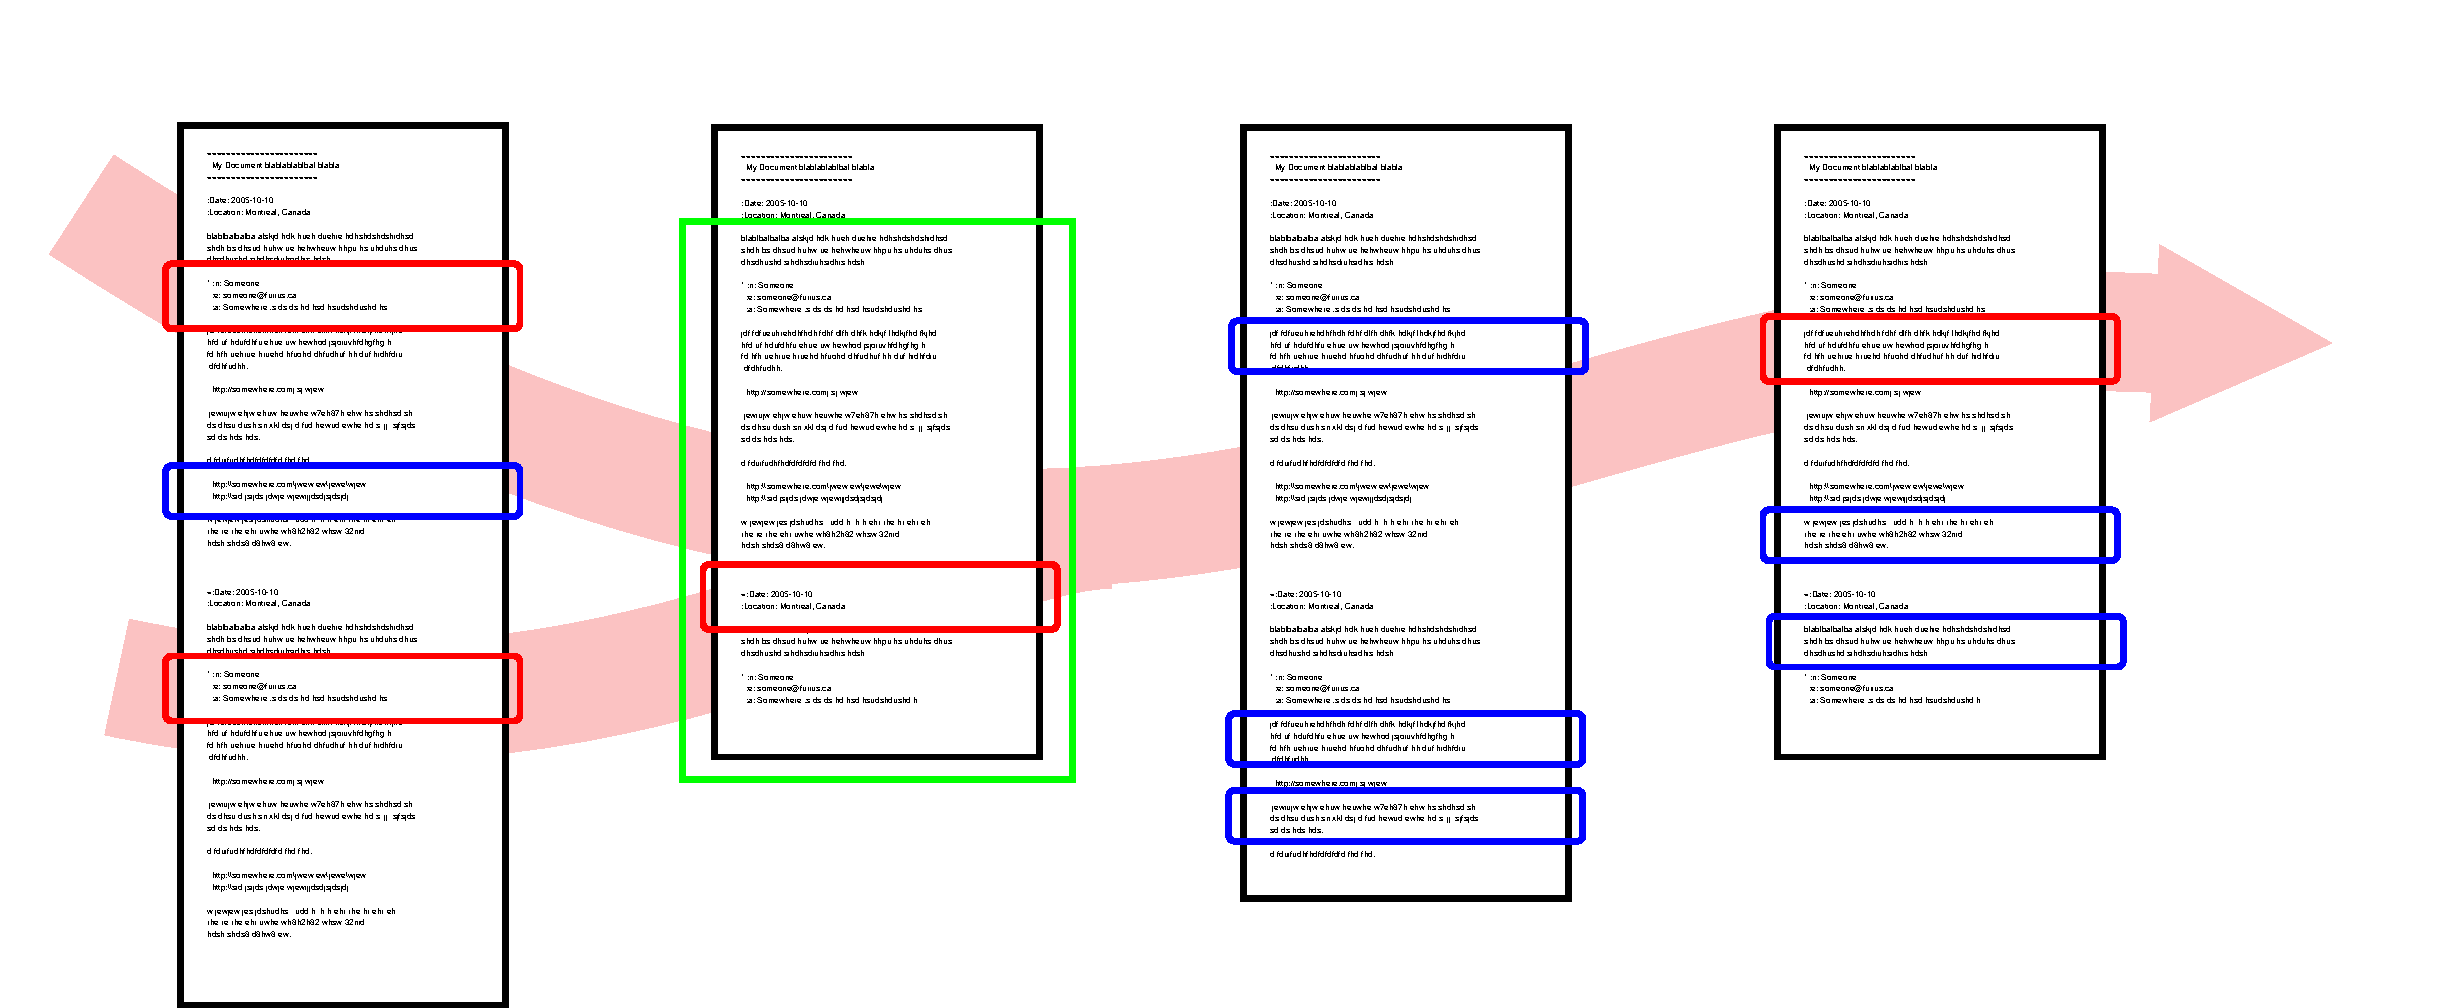
\includegraphics[width=1.0\textwidth]{across3.pdf}

\end{frame}


%-------------------------------------------------------------------------------
\begin{frame}[fragile]
  \frametitle{Data Across Documents}

  What if I could \emph{identify} and \emph{extract} the meaningful parts from
  those files and store them appropriately?  What could I build with this?

\vfill\pause

  You may have heard this idea before: the Semantic Web
  \begin{itemize}
  \item In an ideal world, HTML authors would identify all relevant parts of
    their documents with appropriate markup

  \item You would then be able to create e.g. the ``yellow pages'' of the entire
    internet

  \item Search engines are taking a stab at this holy grail

  \end{itemize}

  But I want this \textbf{now}, and for just my personal corpus of files, even
  if it's a restricted version of this idea.  I want a database built from the
  files on my computer to feed a website, like a blog on steroids.

\end{frame}


%-------------------------------------------------------------------------------
\begin{frame}[fragile]
  \frametitle{The Goal}

  Build a system that can extract semantically meaningful informations in my set
  of personal info files and store them in a structured way (in database
  tables), so I can use this information later and serve in new, interesting
  ways.

\vfill

  Nabu is a Python library that allows you to do that.
  \begin{itemize}
  \item It is not tied specifically to PIM info
  \item You can write extractors for anything, you just have to select the
    docutils structures and conventions that you are going to recognize
  \item On the client it requires only Python to publish files
  \end{itemize}

%   If I had served you this definition in the first place, I'm not sure you
%   would be sitting here.

\end{frame}


%-------------------------------------------------------------------------------
\begin{frame}[fragile]
  \frametitle{Components / Overview}

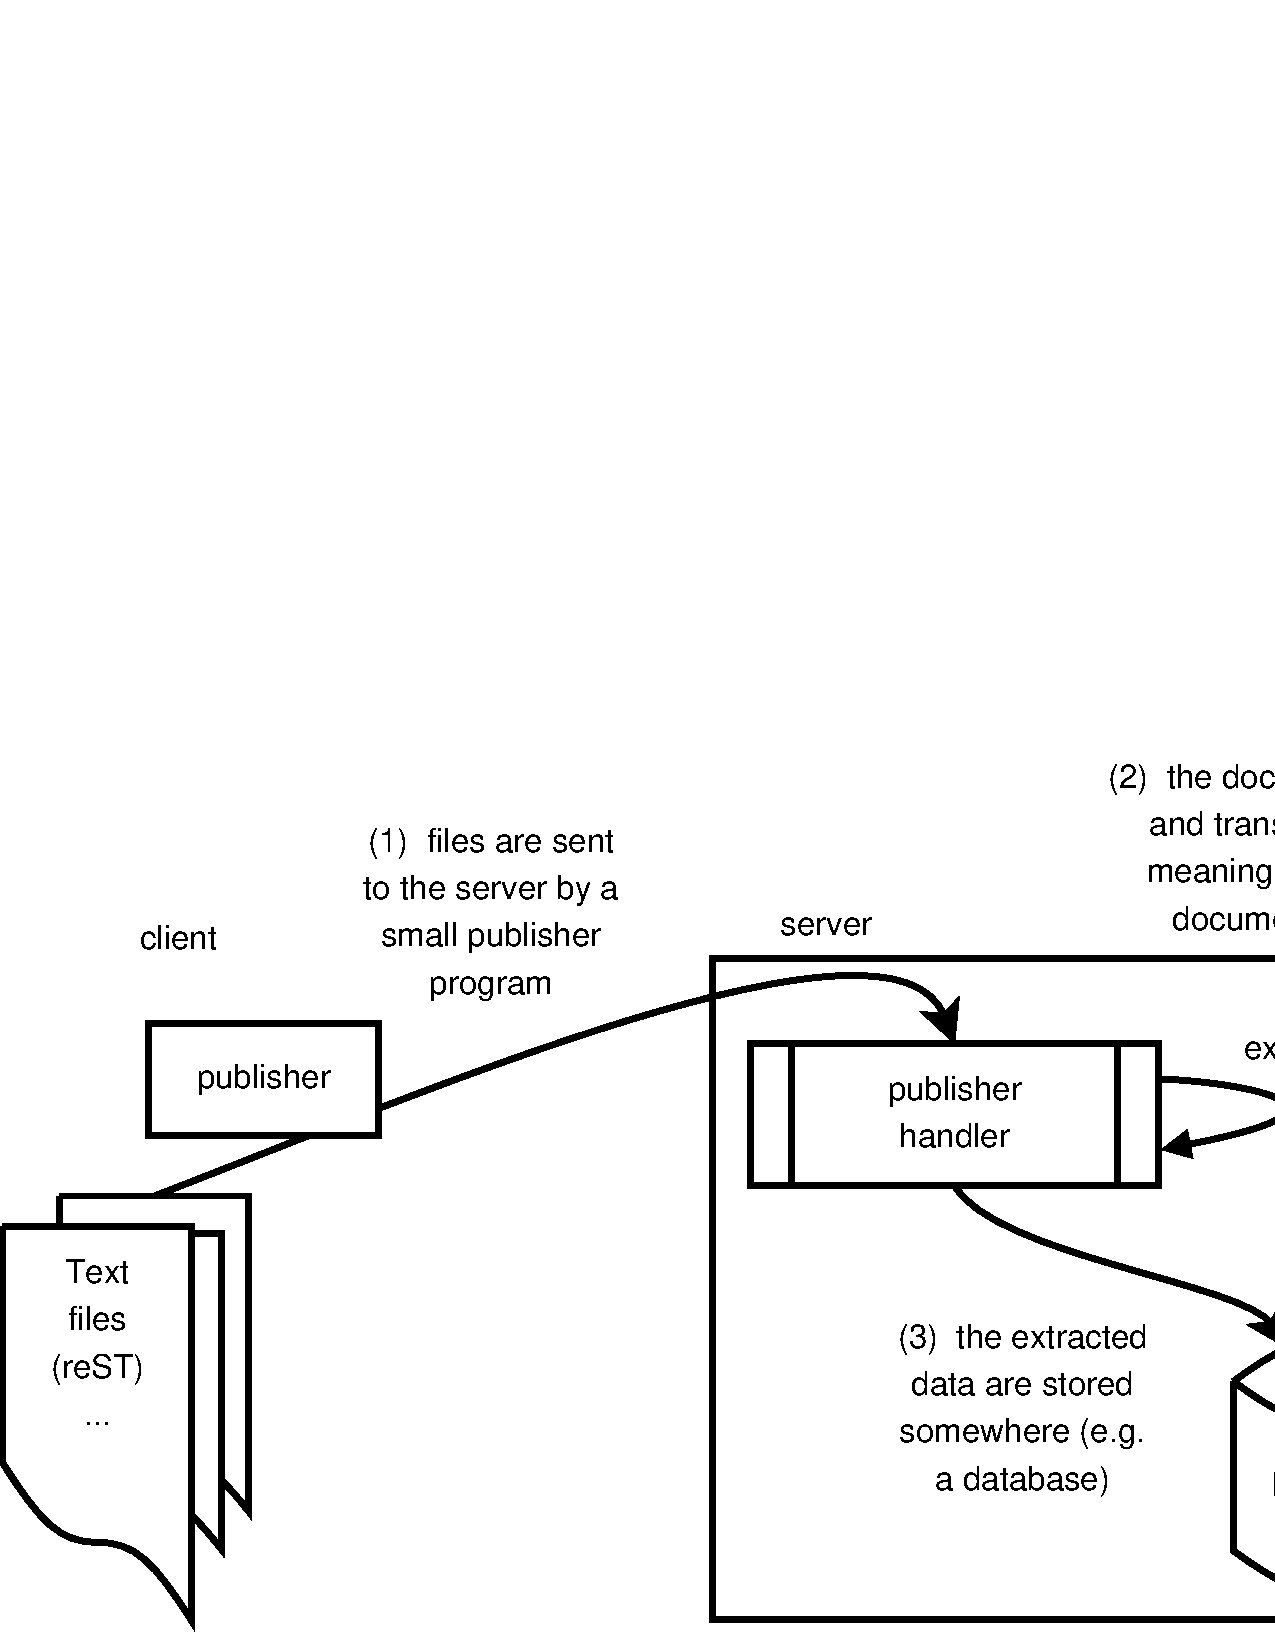
\includegraphics[width=1.0\textwidth]{../nabu2.pdf}

\end{frame}


%-------------------------------------------------------------------------------
\begin{frame}[fragile]
  \frametitle{Components}

  \begin{itemize}
  \item Nabu Publisher Client: searches the files on the client side and sends
    the modified ones to the server
    \begin{itemize}
    \item It fetches MD5 sums from the server and compares the local files
    \item Files are identifies by an embedded Id, so file locations don't matter
\begin{verbatim}
   :Id: 8844db51-36ee-4e2a-8255-84e804f5cbe2
\end{verbatim}
    \end{itemize}

  \item Nabu Server: receives the files, parses them through docutils and runs
    the configured extractors, thereby storing the data

  \item Storage: typically, your database server \\
    (or files or anything else if you like)

  \item Presentation: that's your own thing \\
     (Nabu does not provide presentation)

  \end{itemize}

\end{frame}


%-------------------------------------------------------------------------------
\begin{frame}[fragile]
  \frametitle{Design}

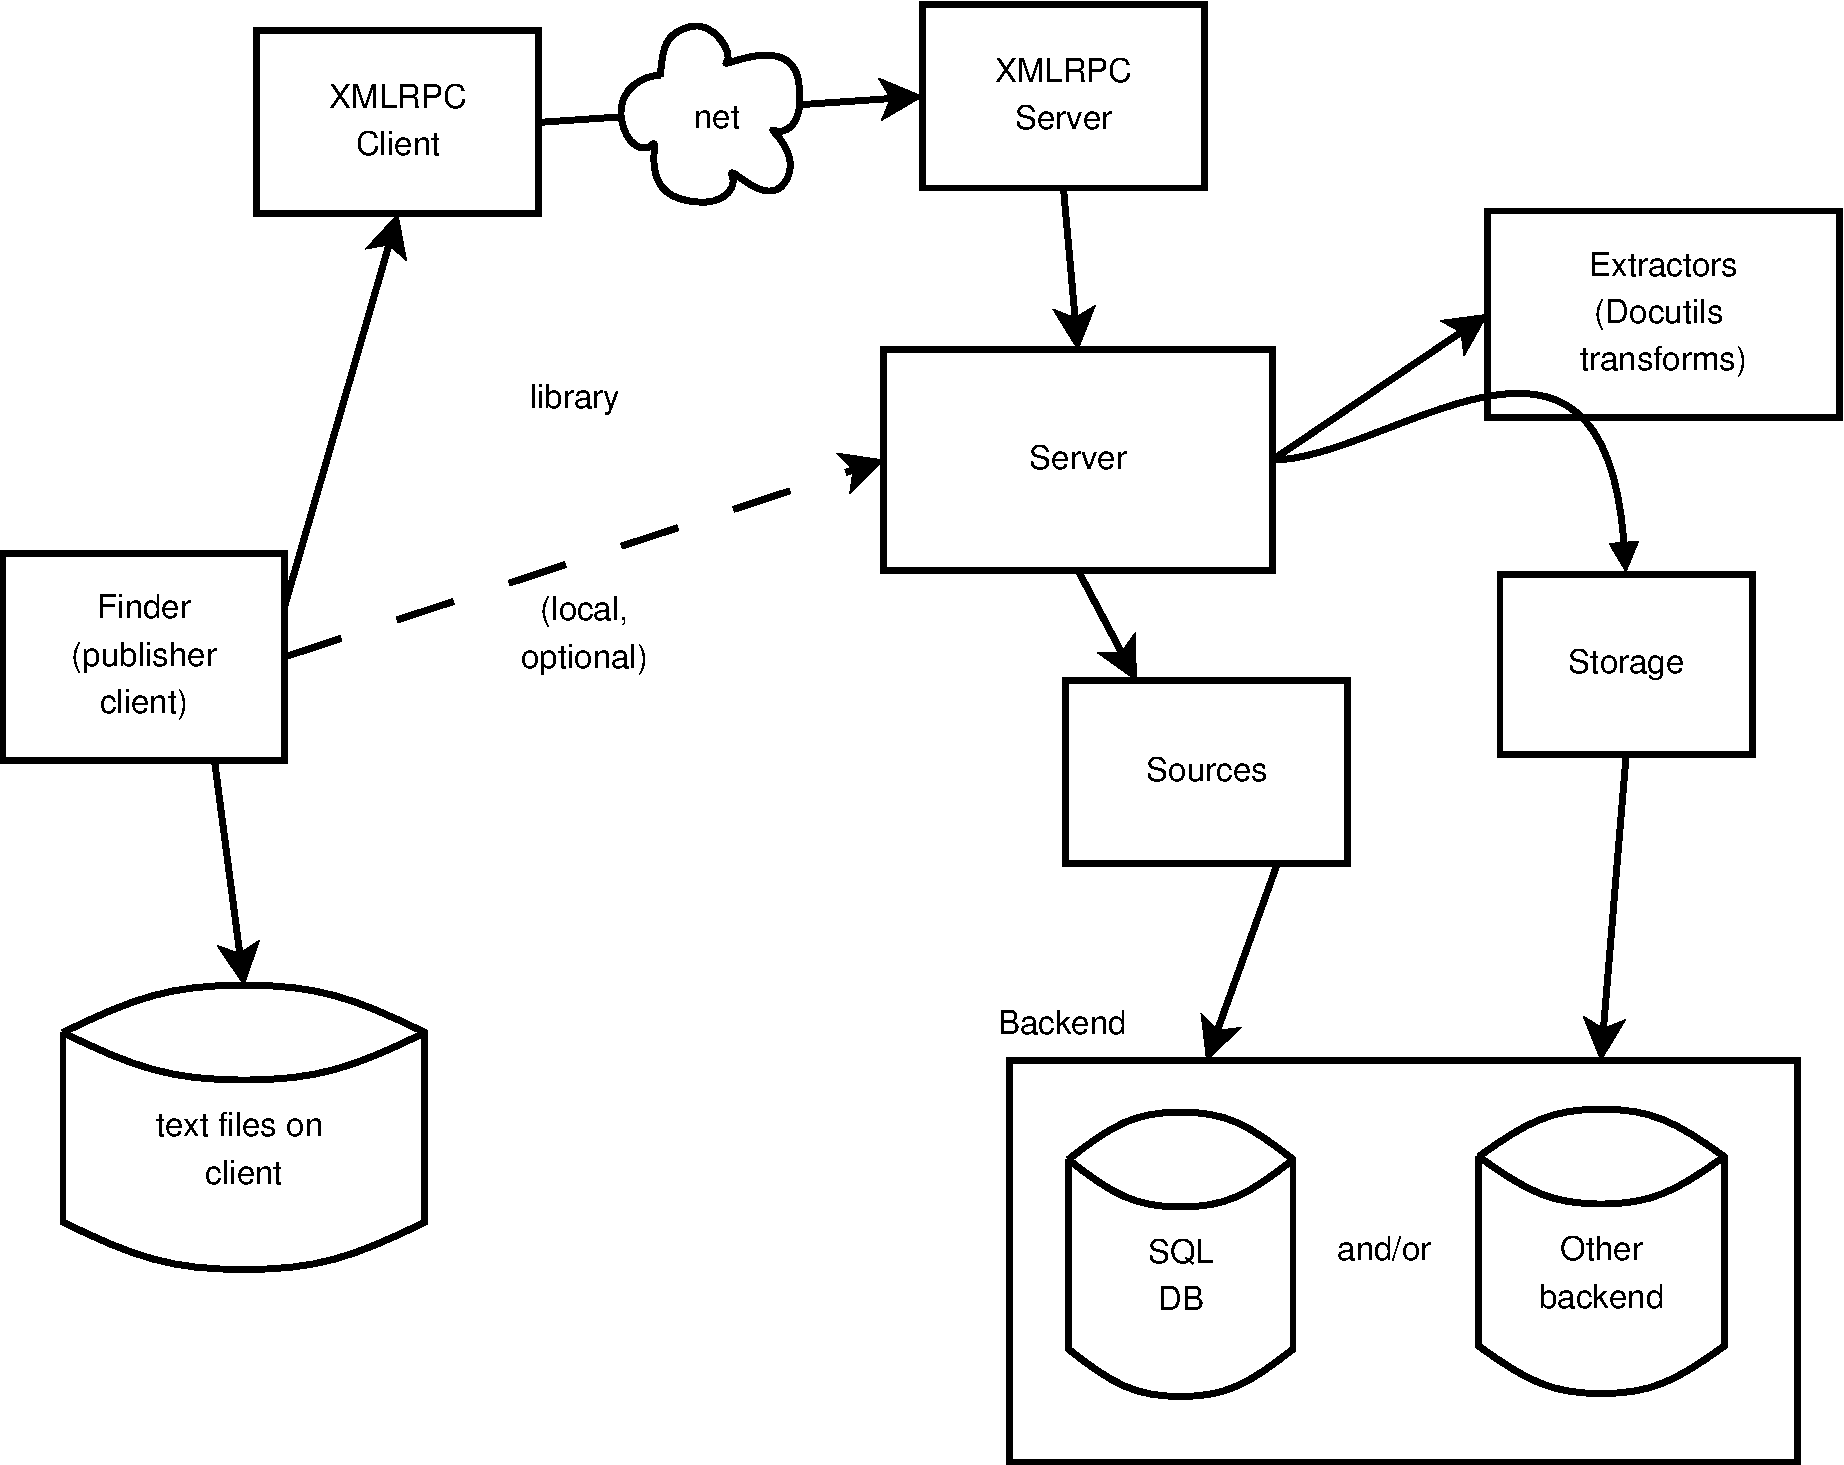
\includegraphics[width=0.9\textwidth]{../nabu1.pdf}

\end{frame}


%-------------------------------------------------------------------------------
\begin{frame}[fragile]
  \frametitle{Extractors}

  You need to write extractors for the stuff that you are interested in, for
  example:

{\scriptsize
\begin{verbatim}
  * :name: Bill Gates
    :email: billg@microsoft.com
\end{verbatim}
}

\vfill

  Use \texttt{rst2pseudoxml.py} to figure how docutils parses it:

{\scriptsize
\begin{verbatim}
<bullet_list bullet="*">
    <list_item>
        <field_list>
            <field>
                <field_name>
                    name
                <field_body>
                    <paragraph>
                        Bill Gates
            <field>
                <field_name>
                    email
                <field_body>
                    <paragraph>
                        <reference refuri="mailto:billg@microsoft.com">
                            billg@microsoft.com
\end{verbatim}
}

\end{frame}


%-------------------------------------------------------------------------------
\begin{frame}[fragile]
  \frametitle{Extractors}

{\small
Then implement it:
\begin{verbatim}
class AddressExtractor(extract.Extractor):

    def apply( self, **kwargs ):
        v = AddressVisitor(self, self.document)
        self.document.walkabout(v)

class AddressVisitor(...):
    ...

class AddressStorage(extract.SQLExtractorStorage):

    def store( self, unid, name, tfields ):
    ... # store the stuff in a database

\end{verbatim}
%    default_priority = 900
}

\end{frame}


%-------------------------------------------------------------------------------
\begin{frame}[fragile]
  \frametitle{Target Audience}

{\large\begin{center}
\textbf{It's not for your mom!}
\end{center}}

  It is intended only for people who have developed the ability to edit text
  files carefully (typically programmers, you guys).

 \begin{itemize}
 \item We understand indentation
 \item We know about spacing, justification, filling, etc.
 \item We are careful about pesky little details
 \item This is what makes creating ReST files possible
 \end{itemize}

\vfill

  I want to leverage this ability!

\end{frame}





% before ?

%-------------------------------------------------------------------------------
\begin{frame}[fragile]
  \frametitle{ReStructuredText and docutils}

  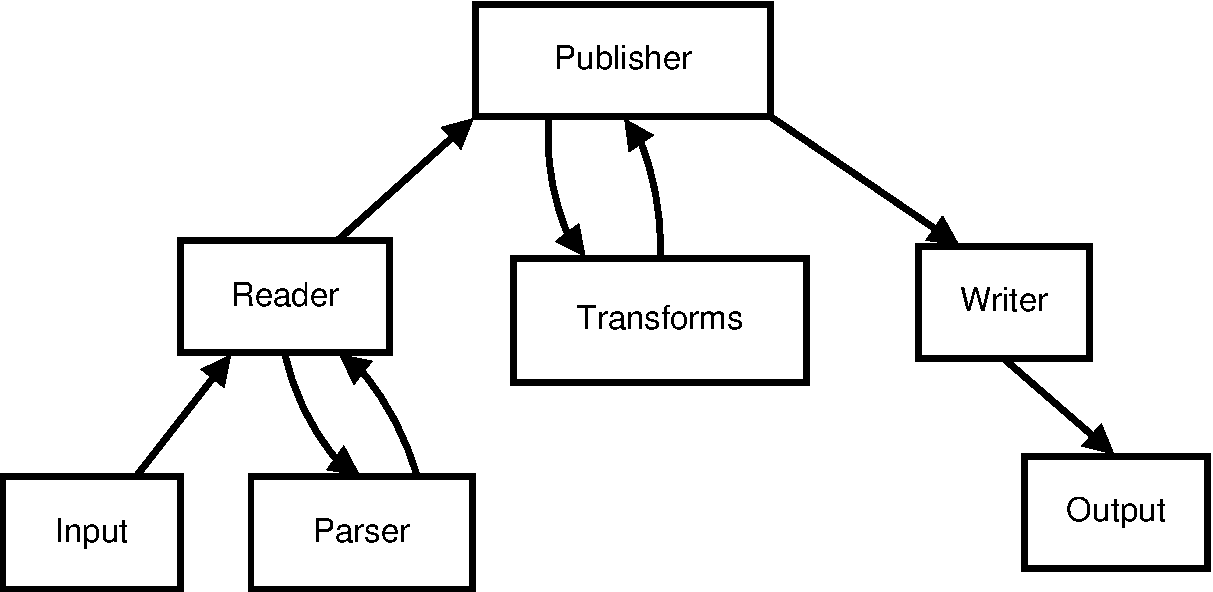
\includegraphics[width=1.0\textwidth]{docutils1.pdf}

\end{frame}


%-------------------------------------------------------------------------------
\begin{frame}[fragile]
  \frametitle{ReStructuredText and docutils}

  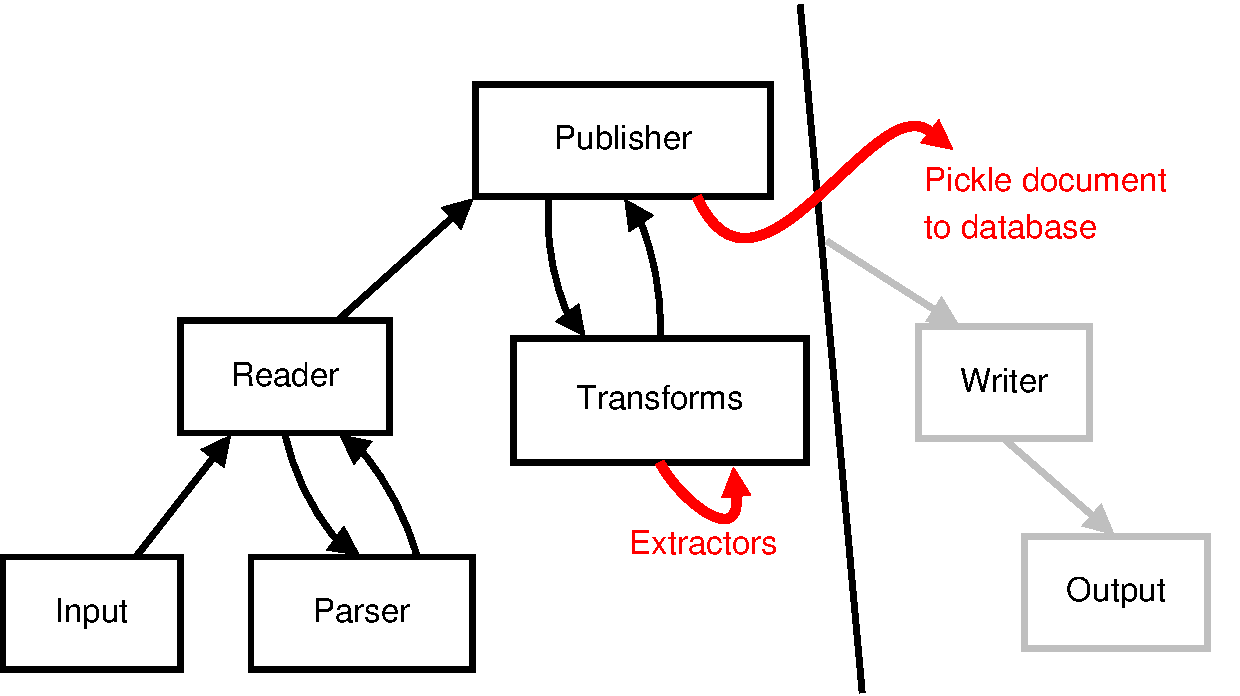
\includegraphics[width=1.0\textwidth]{docutils2.pdf}

\end{frame}

% ReStructuredText
% ================
%
% .. ask Goodger to get up
%
%    "If you see this guy in the corridor, show him some love, give him a hug."
%
% - The best text-to-structure conversion tool.
% - Finds the best compromises (all decisions are documented thoroughly)
%
%
% .. <show some text with recursive boxes in it>
%

% FIXME: build a graph with the docutils structure, the one with
% reader/transform/writer, same as in the documentation, with the intention to

% explain that I've had to modify it and to stop the process halfway and that I
% store this document in pickled format













%-------------------------------------------------------------------------------
\begin{frame}[fragile]
  \frametitle{Document Presentation Example}

  \begin{center}
    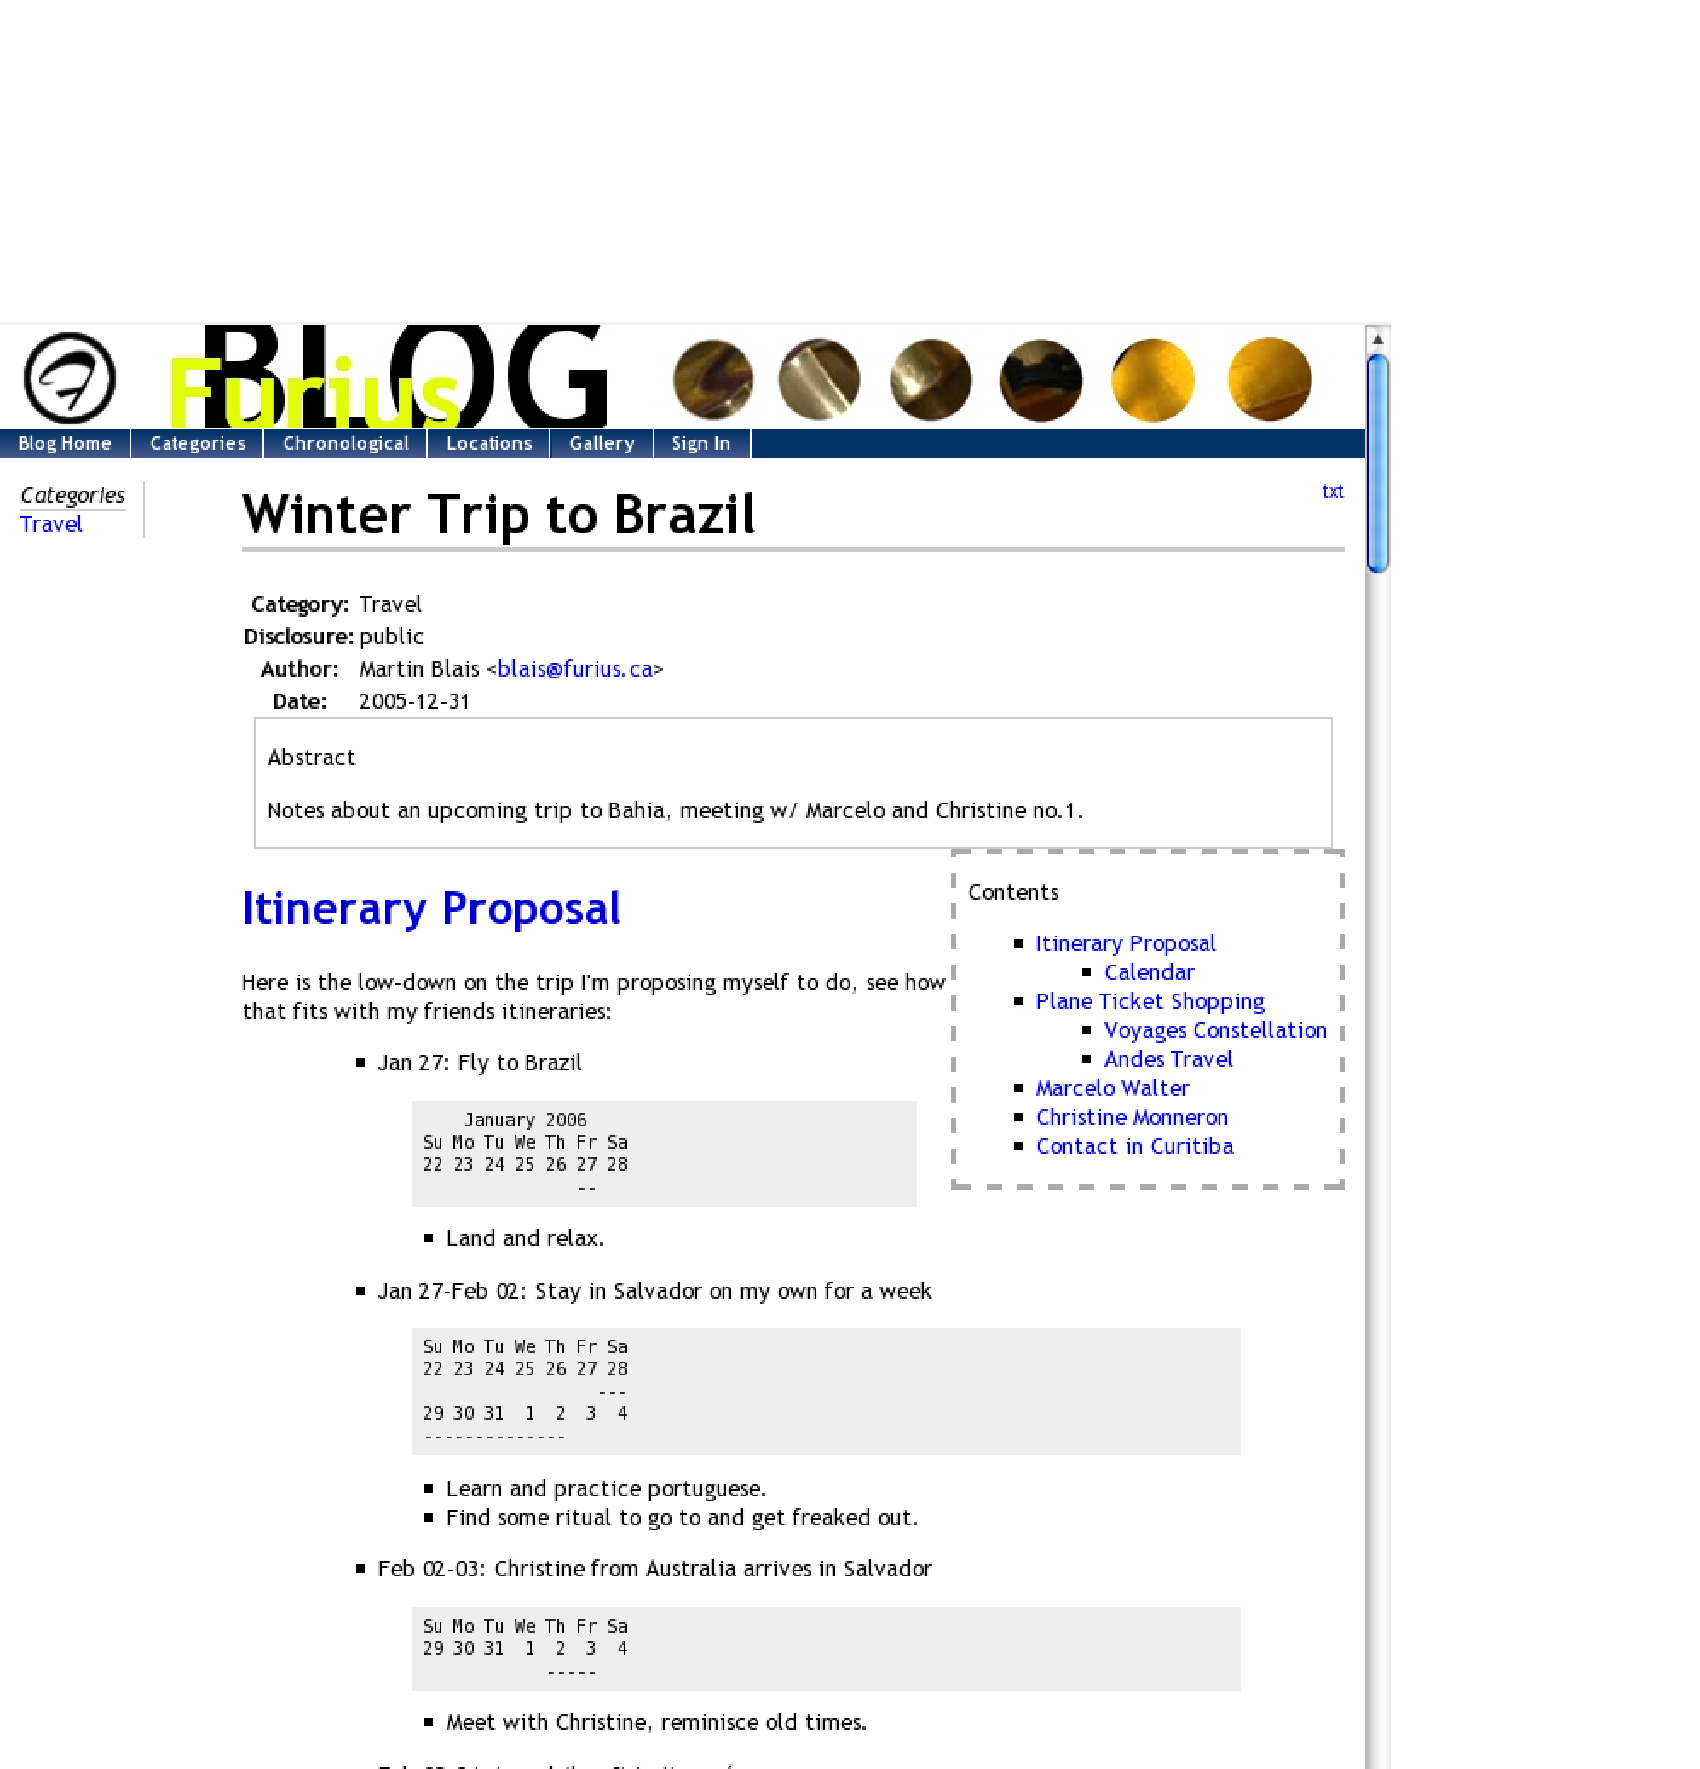
\includegraphics[width=0.7\textwidth]{page-shot.pdf}
  \end{center}

\end{frame}


%-------------------------------------------------------------------------------
\begin{frame}[fragile]
  \frametitle{Events Example}

{\small
\begin{verbatim}
sat 2005-12-31 19h30
  - NYE Evening chez Stuart

sat 2005-12-31
  - Proteus: mkisofs for backup copy DVD-ROM

2006-01-02
  - Contact SonoMax about free earplugs
  - Track Leif's grille that was supposed to arrive.

2006-01-03
  - Visit Yves * D'ailleurs je vais avoir besoin de tes info pour les
    salaires de 2005

  - Confirm flight to Brazil w/ Constellation

2006-01-04 20h00
  - Dinner w/ Pierre @ Golden Cari

2006-01-05
  - Book room for PyCon (should be 79 USD) in january when problems are fixed.

2006-01-13, 14, 16
  - Vote par anticipation

\end{verbatim}
}

\end{frame}


%-------------------------------------------------------------------------------
\begin{frame}[fragile]
  \frametitle{Events Example}
  \framesubtitle{Calendar View}

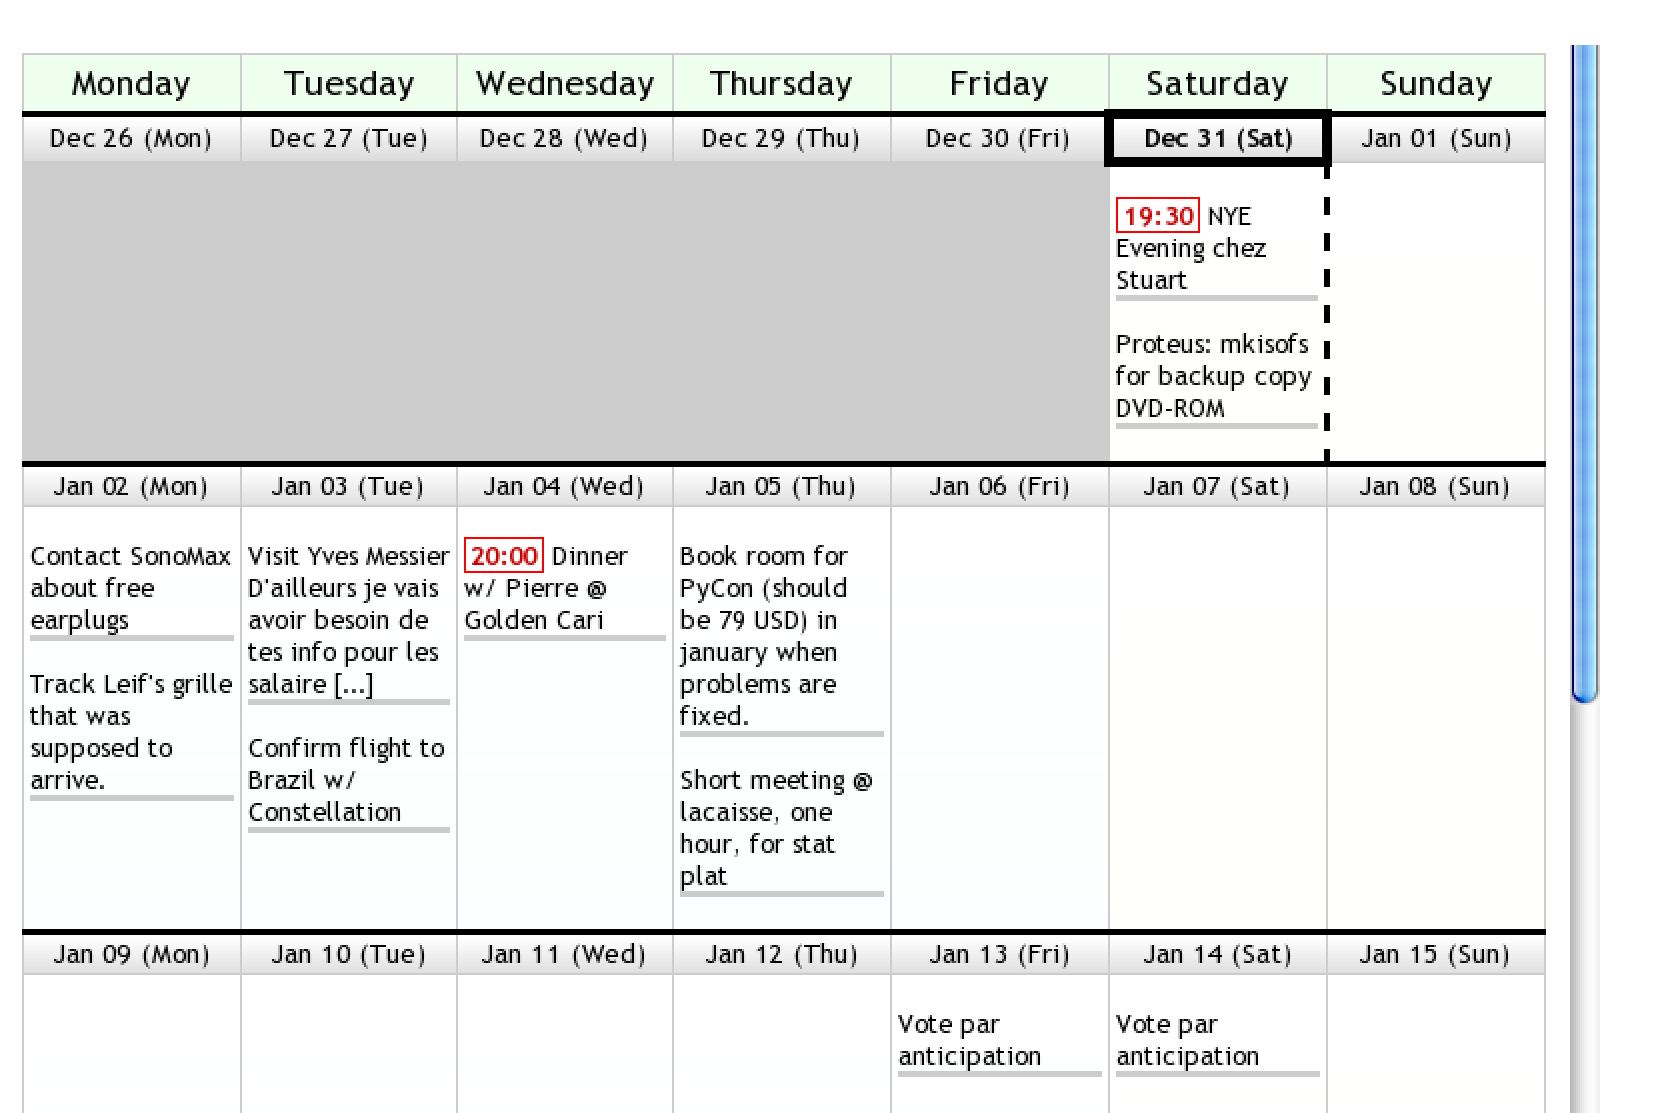
\includegraphics[width=1.0\textwidth]{calendar-shot.pdf}

% Add this: I have dated events in my file for Brazil, PyCon, my TODO file, they
% all merge into my calendar.

\end{frame}



%-------------------------------------------------------------------------------
\begin{frame}[fragile]
  \frametitle{Other Examples}

  \begin{itemize}
  \item Billing info: you could define a simple timesheet format in a text file
    and have some kind per-task or per-client billing info page

  \item Dynamic website data: you could use Nabu to feed some data for a web
    site, this allows you to avoid having to write input forms

  \end{itemize}

\end{frame}


%-------------------------------------------------------------------------------
\begin{frame}[fragile]
  \frametitle{Nabu Contents Browser - Extracted}

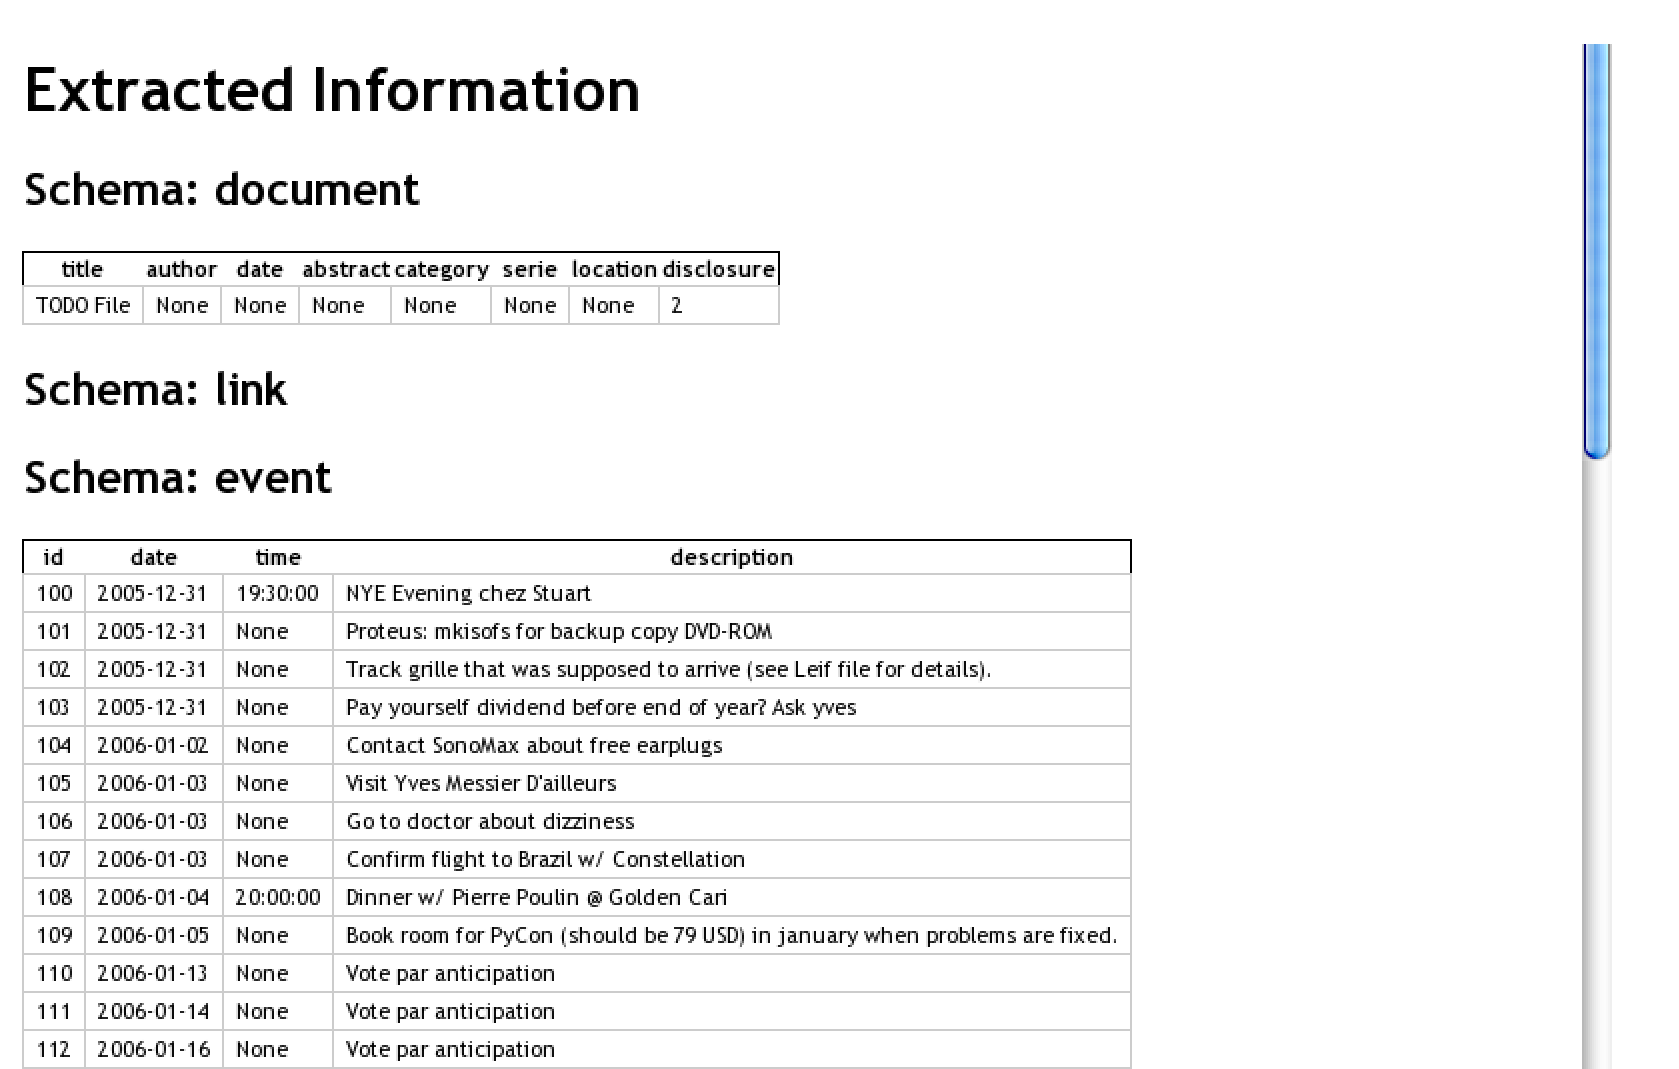
\includegraphics[width=1.0\textwidth]{ll-extracted.pdf}

\end{frame}


%-------------------------------------------------------------------------------
\begin{frame}[fragile]
  \frametitle{Nabu Contents Browser - Upload Info}

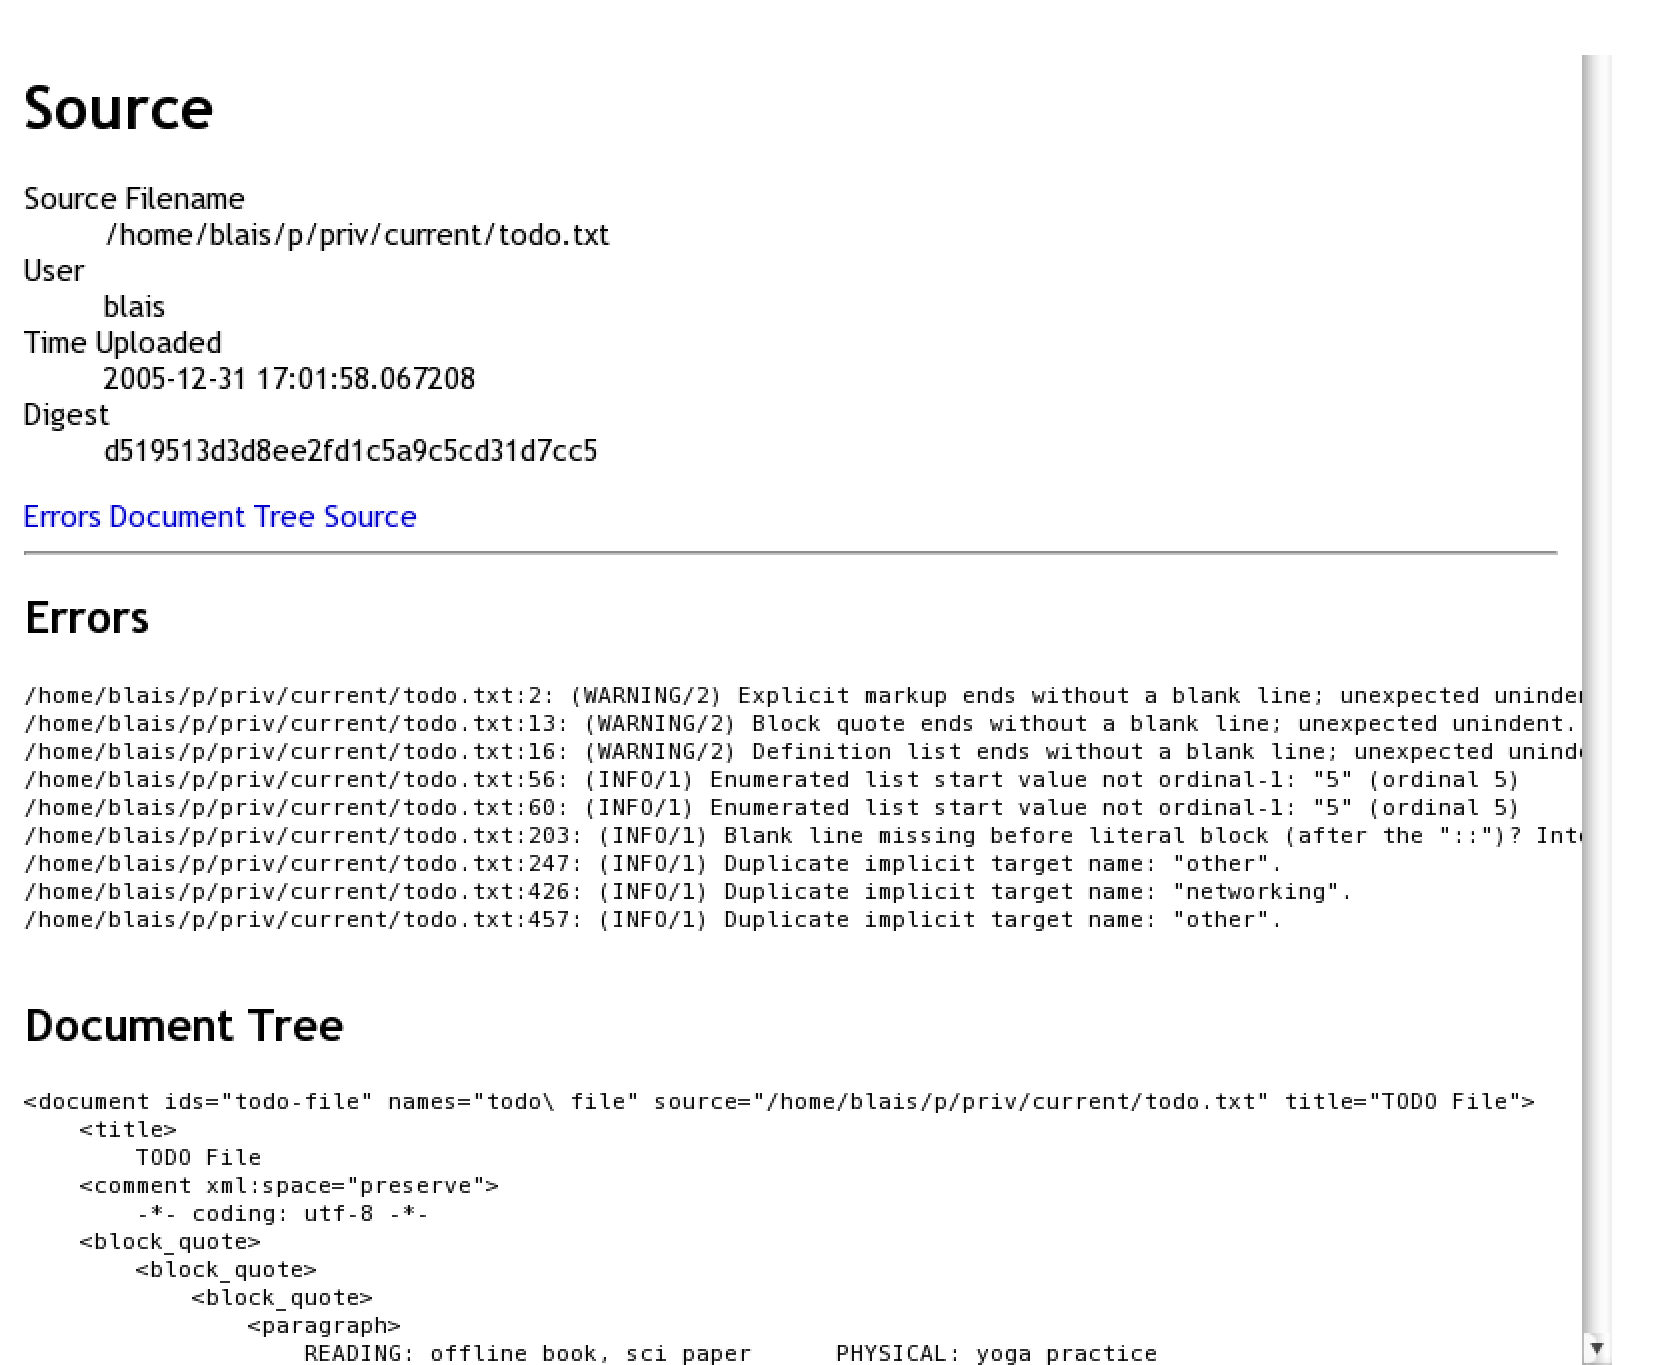
\includegraphics[width=1.0\textwidth]{ll-upload.pdf}

\end{frame}





%-------------------------------------------------------------------------------
\begin{frame}[fragile]
  \frametitle{Problems}

- Creating precise reStructuredText can be fragile from the user's point-of-view

- you need to make sure that your set of Ids are unique
  - use UUIDs (78d8a600-abb4-49c0-a0fc-1c315cddbc1a)

- You end up getting dragged into the docutils project a bit

(EXAMPLE)

% - You have to understand how restructuredtext gets parsed
%
%   - You end up getting dragged into the docutils project a bit
%
%   --> You can use rst2pseudoxml.py to easily debug and learn input syntaxes

\end{frame}


%-------------------------------------------------------------------------------
\begin{frame}[fragile]
  \frametitle{Future Work}

  \begin{itemize}
  \item Stabilize (I need to finish my own presentation layer)
  \item Support encryption in the publisher client
  \item Support per-document options
  \end{itemize}

\end{frame}


%-------------------------------------------------------------------------------
\begin{frame}[fragile]
  \frametitle{Questions}

{\LARGE
  \begin{center}
Nabu homepage:\\
\verb=http://furius.ca/nabu/=
  \end{center}
}

\end{frame}


%===============================================================================
\end{document}




% Add: MapExtractor that can extract all my links to Google maps and create a
% single map with them, or a list of locations, they could be accompanied with a
% trail, and then each trail be displayed separately





% You need to talk about sharing a corpus of documents between users

% mention something about a Subversion hook




% * borrow someone's mouse for the show
% * use xannotate during the presentation






% TODO: explain how the extracted data gets REPLACED whenever a document is
% uploaded
